%%Mathematics-----------------------------------------
\section{Mathematics}

The text below is not a rigorous approach to the mathematical theory, nor is it a wholly systematic or comprehensive description of the topics covered. It is a selection of topics recommended by core instructors. These include mathematical concepts and procedures that will be encountered in your core courses, and instructors expect you to be familiar with them prior to the beginning of a course, i.e, they will not cover them in detail. Instead, use the content below as a reference as these topics arise and as a platform for more in-depth study. Please contact \href{mailto:jonathan.emery@northwestern.edu}{jonathan.emery@northwestern.edu} with suggestions for additional material to be included in this section.

For those who have never seen the mathematics below or who are not comfortable with the material, further preparation may be necessary. Options for those students include: either a.) enroll in ES-APPM-311-1 and ES-APPM-311-2: Methods of Applied Mathematics and/or b.) utilizing the suggested resources for supplemental study.

\subsection{Linear Algebra}

Linear algebra is a branch of mathematics that is central to physical description in Materials Science as it concerns the description of vectors spaces and is used in solving systems of equations. Materials Science graduate students will encounter application of linear algebra in all core courses. The sections below outline basic linear algebra concepts. \ignore{Refer to \ref{App:AppendixB} for}

\subsubsection{Linear Systems}
\subsubsection{Gauss Elimination \hfill (Release TBD)}
\subsubsection{Matrix Algebra and Operations \hfill (Release TBD)}
\subsubsection{Linear Transformations \hfill (Release TBD)}
\subsubsection{Determinants \hfill (Release TBD)}
\subsubsection{Eigenvalues and Eigenvectors \hfill (Release TBD)}
\subsubsection{Linear Differential Equations \hfill (Release TBD)}
	\begin{enumerate}
		\item Linear Differential Operators
		\item Linear Differential Equations
	\end{enumerate}




\pagebreak
\subsection{Tensors \hfill(Release 1/2017)}\label{subsec:Tensors}

Tensors are mathematical objects that define relationships between scalars, vectors, matrices, and other tensors. Tensors are represented as \textit{arrays} of various dimensionality (defined by rank or order). The moniker ``tensor'' in general suggests a higher-rank array (most often $\geq$3 dimensions), but scalars, vectors, and matrices are also tensors.

In the MSE graduate core, students will encounter tensors of various rank. In physical science, tensors characterize the properties of a physical system. Tensors are the \textit{de facto} tool used to describe, for example, diffusion, nucleation and growth, states of stress and strain, Hamiltonians in quantum mechanics, and many, many, more physical phenomenon. Physical processes of interest to Materials Scientists take place in Euclidean 3-space (${\rm I\!R}^3$) are are well-described by tensor representations.

We build up our description of the handling of tensors starting by separately describing rank-0, rank-1, rank-2, and rank-3 tensors. Tensors of lower ranks should be familiar --- students will have encountered them previously as scalars (rank-0), vectors (rank-1), and matrices (rank-2). The term \emph{tensors} typically denotes arrays of higher dimensionality (rank $\geq3$). Physical examples include the rank-2 \href{https://en.wikipedia.org/wiki/Cauchy_stress_tensor}{Cauchy stress tensor} which describes the stress state of a at a point within a material), the rank-3 piezoelectric tensor (which relates the dielectric polarization of a material to a stress state), and the rank-4 stiffness tensor (which relates strain state and stress state in a system that obeying Hooke's law).

Classifications of tensors by  rank allows us to quickly identify the number of tensor components we will work with: a tensor of order $p$ has $N^p$ components, where $N$ is the dimensionality of space in which we are operating. In general, you will be operating in Eucledian 3-space, so the number of components of a tensor is defined as $3^p$. 

\paragraph{Scalars}are considered tensors with \emph{order} or \emph{rank} of 0. Scalars represent physical quantities (often accompanied by a unit of measurement) that possess only a magnitude: e.g., temperature, mass, charge, and distance. Scalars are typically represented by Latin or Greek symbols and have $3^{0} = 1$ component.

\paragraph{Vectors}are tensors with a \emph{rank} of 1. In symbolic notation, vectors are typically represented using lowercase bold or bold-italic symbols such as $\mathbf{u}$ or $\pmb{a}$. Bold typeface is not always amenable to handwriting, however, and so the a right arrow accent is employed: $\vec{u}$ or $\vec{a}$.  Students are likely to encounter various conventions depending on their field of study.

In ${\rm I\!R}^3$ a vector is defined by $3^{1} = 3$ components. In \textit{xyz} Cartesian coordinates we utilize the Cartesian basis with 3 orthogonal unit vectors $\{\mathbf{e}_{\mathbf{x}}\text{, } \mathbf{e}_{\mathbf{y}}\text{, } \mathbf{e}_{\mathbf{z}}\}$. We define 3D vector $\mathbf{u}$ in this basis with the components ($u_x$, $u_y$, $u_z$), or equivalently  ($u_1$, $u_2$, $u_3$). Often, we represent the vector $\mathbf{u}$ using the shorthand $u_i$, where the $i$ subscript denotes an index that ranges over the dimensionality of the system (1,2,3 for ${\rm I\!R}^3$, 1,2 for ${\rm I\!R}^2$). %Need to figure out \bm!

Vectors are often encountered in a bracketed vertical list to facilitate matrix operations. Using some of the notation defined above:

\begin{equation}
\mathbf{u} = u_i = 
	\begin{bmatrix}
    u_x \\
    u_y \\
    u_z
	\end{bmatrix} =
	\begin{bmatrix}
    u_1 \\
    u_2 \\
    u_3
	\end{bmatrix}
	\label{eq:Vector}
\end{equation}

\paragraph{Matrices}are tensors with a \emph{rank} of 2.  In ${\rm I\!R}^2$ a matrix has $2^{2} = 4$ components and in ${\rm I\!R}^3$ a matrix has $3^{2} = 9$ components. As with vectors, we will use the range convention when denoting a matrix, which now possesses two subscripts, $i$ and $j$. We use the example of the true stress, or \href{https://en.wikipedia.org/wiki/Cauchy_stress_tensor}{Cauchy stress tensor}, $\sigma_{ij}$:

\begin{equation}
\sigma_{ij} =  
	\begin{bmatrix}
    \sigma_{xx} & \sigma_{xy} & \sigma_{xz}\\
    \sigma_{yx} & \sigma_{yy} & \sigma_{yz}\\
    \sigma_{zx} & \sigma_{zy} & \sigma_{zz}\\
	\end{bmatrix}
\end{equation}

Where the diagonal represents the normal components of stress and the off-diagonal represents the shear components of the stress. In this notation the first index denotes the row while the second denotes the column ($x = 1$, $y = 2$, $z = 3$).

\paragraph{Tensors} A rank-3 tensor in ${\rm I\!R}^3$ has $3^{3} = 27$ components and is represented in range notation using subscripts $i$, $j$, and $k$, e.g., $T_{ijk}$ . At rank-3 (and it is even worse in rank-4, requiring an array of rank-3 tensors) it begins to become difficult to represent clearly on paper. An example of a simple tensor --- \href{https://en.wikipedia.org/wiki/Levi-Civita_symbol#Three_dimensions_2}{the rank-3 permutation tensor} --- is shown in Fig. \ref{fig:PermutationTensor}. You can also watch \href{https://www.youtube.com/watch?v=f5liqUk0ZTw}{this video} which helps with the visualization. 

\begin{figure}%
	\centering
	\includegraphics[scale=0.5]{PermutationTensor}%
	\caption{The rank-3 permutation tensor, by Arian Kriesch. corrections made by Xmaster1123 and Luxo (Own work) [GFDL (http://www.gnu.org/copyleft/fdl.html), CC-BY-SA-3.0 (http://creativecommons.org/licenses/by-sa/3.0/)}%
	\label{fig:PermutationTensor}%
\end{figure}

One can write the $i = 1,2,3$ matrices that stack to form this tensor as: %This should be replaced as just a general tensor. I can adapt the tensor.

\begin{equation}
	\epsilon_{1jk}=
	\begin{bmatrix}
		0 & 0 & 0\\
		0 & 0 & 1\\
		0 & -1 & 0
	\end{bmatrix}
\end{equation}

\begin{equation}
	\epsilon_{2jk}=
	\begin{bmatrix}
		0 & 0 & -1\\
		0 & 0 & 0\\
		1 & 0 & 0
	\end{bmatrix}
\end{equation}

\begin{equation}
	\epsilon_{3jk}=
	\begin{bmatrix}
		0 & 1 & 0\\
		-1 & 0 & 0\\
		0 & 0 & 0
	\end{bmatrix}
\end{equation}




	%\subsubsection{Vector Calculus \hfill(Release TBD)}
	%
	%\textit{\textbf{Encountered in: MAT\texttt{\_}SCI 406, 408}}  \pagebreak
\subsection{Summation Notation}\label{sec:SummationNotation}

Often, it is useful to simplify notation when manipulating tensor equations. To do this, we utilize Einstein summation notation, or simply \emph{summation notation}. This notation says that \emph{if an index is repeated twice (and only twice) in a single term we assume summation over the range of the repeated subscript}. The simplest example of this is the representation of the trace of a matrix:

\[tr(\sigma) = \underbrace{\sigma_{kk}}_{\substack{\text{summation} \\ \text{notation}}} = \sum_{k}^{3}\sigma_{kk} = \sigma_{11}+\sigma_{22}+\sigma_{33}\]

In $\sigma_{kk}$ the index $k$ is repeated, and this means that we assume summation of the index over the range of the subscript (in this case, 1-3 as we are working with the stress tensor).

\begin{displayquote}
	\textbf{Example 1:}This comes in very useful when representing matrix multiplication. Let's say we have an ($M \times N$) matrix, $\mathbf{A} = a_{ij}$ and an $R \times P$ matrix $\mathbf{B} = b_{ij}$. We know from linear algebra that the matrix product $\mathbf{AB}$ is defined only when $R = N$, and the result is a ($M \times P$) matrix, $\mathbf{C} = c_{ij}$. Here's an example with a ($2 \times 3$) matrix times a ($3 \times 2$) in conventional representation:

\begin{align*}
\mathbf{AB} =
	\begin{bmatrix}
		a_{11} & a_{12} & a_{13}\\
		a_{21} & a_{22} & a_{23}\\
	\end{bmatrix}
	&\begin{bmatrix}
		b_{11} & b_{12}\\
		b_{21} & b_{22}\\
		b_{31} & b_{32}\\
	\end{bmatrix}
	= \\
	&\begin{bmatrix}
		a_{11}b_{11} + a_{12}b_{21} + a_{13}b_{31} & a_{11}b_{12} + a_{12}b_{22} + a_{13}b_{32}\\
		a_{21}b_{11} + a_{22}b_{21} + a_{23}b_{31} & a_{21}b_{12} + a_{22}b_{22} + a_{23}b_{32}\\
	\end{bmatrix}
	=c_{ij}
\end{align*}

Here, we can use summation notation to greatly simply the expression. The components of the matrix $c_{ij}$ are $c_{11}$, $c_{12}$, $c_{21}$, and $c_{22}$ and are defined:

\begin{align*}
	c_{11} = a_{11}b_{11} + a_{12}b_{21} + a_{13}b_{31}\\
	c_{12} = a_{11}b_{12} + a_{12}b_{22} + a_{13}b_{32}\\
	c_{21} = a_{21}b_{11} + a_{22}b_{21} + a_{23}b_{31}\\
	c_{22} = a_{21}b_{12} + a_{22}b_{22} + a_{23}b_{32}\\
\end{align*} 

These terms can all be represented using the following expression:

\begin{equation}
	c_{ij} = \sum_{k=1}^{3} a_{ik}b_{kj} = a_{i1}b_{1j} + a_{i2}b_{2j} + a_{i3}b_{3j}
\end{equation}

So, in general for any matrix product:

\begin{equation}
	c_{ij} = \sum_{k=1}^{N} a_{ik}b_{kj} = a_{i1}b_{1j} + a_{i2}b_{2j} + \cdots +  a_{iN}b_{Nj}
	\label{eq:MatrixMultiply}
\end{equation}

Or, by dropping the summation symbol and fully utilizing the summation convention:

\begin{equation}
	c_{ij} = a_{ik}b_{ki}
\end{equation}

Note that the term $c_{ij}$ \emph{has no repeated subscript - there is no summation implied here. It is simply a matrix}. Summation \emph{is} implied in the $a_{ik}b_{kj}$ term because of the repeated index $k$, often called the dummy index.
\end{displayquote}

\begin{displayquote}
	\textbf{Example 2:} Another example is a $3 \times 3$ matrix multiplied by a (3 \times 1) column vector:

\begin{equation}
	\begin{bmatrix}
		a_{11} & a_{12} & a_{13}\\
		a_{21} & a_{22} & a_{23}\\
		a_{31} & a_{32} & a_{33}\\
	\end{bmatrix}
	\begin{bmatrix}
		b_1\\
		b_2\\
		b_3\\
	\end{bmatrix}
	=
	\begin{bmatrix}
		a_{11}b_{1} + a_{12}b_{2} + a_{13}b_{3} \\
		a_{21}b_{1} + a_{22}b_{2} + a_{23}b_{3}\\
		a_{31}b_{1} + a_{32}b_{2} + a_{33}b_{3}\\
	\end{bmatrix}
	= a_{ij}b_{j}
\end{equation}
\end{displayquote}

\begin{table}%
	\centering
	\begin{tabularx}{6in}{ccc}
		\toprule
		\pbox{20em}{Summation \\ convention} & \pbox{20em}{Non-summation \\ convention} & Full expression \\
		\midrule
		$\lambda = a_ib_i$ & $\lambda = \sum\limits_{i=1}^{3}a_ib_i$ & $\lambda = a_1b_1 + a_2b_2 + a_3b_3$\\
		\midrule
		$c_i = S_{ik}x_k$ & $c_i = \sum\limits_{i=1}^{3}S_{ik}x_k$ & 
		$c_i = \begin{cases}
			c_1 = S_{11}x_1 + S_{12}x_2 + S_{13}x_3\\ 
			c_2 = S_{21}x_1 + S_{22}x_2 + S_{23}x_3\\
			c_3 = S_{31}x_1 + S_{32}x_2 + S_{33}x_3\\
		\end{cases}$\\
		\midrule
		$\lambda = S_{ij}S_{ij}$ & $\lambda = \sum\limits_{j=1}^{3}\sum\limits_{i=1}^{3}S_{ij}S_{ij}$ & $\lambda = S_{11}S_{11} + S_{12}S_{12} + \cdots + S_{32}S_{32}+S_{33}S_{33}$\\
		\midrule
		$C_{ij} = A_{ik}B_{kj}$ & $\lambda = \sum\limits_{k=1}^{3}A_{ik}B_{kj}$ & $\big[C\big]=\big[A\big]\big[B\big]$\ignore{\footnote{see Eq. \ref{eq:MatrixMultiply} and preceding derivation.}}\\
		\midrule
		$C_{ij} = A_{ki}B_{kj}$ & $\lambda = \sum\limits_{k=1}^{3}A_{ki}B_{kj}$ & $\big[C\big]=\big[A\big]^{T}\big[B\big]$\\
		\bottomrule
	\end{tabularx}
\caption{Uses of summation notation that students may encounter in the graduate core. Bracketed symbols indicate $3 \times 3$ matrices}
\label{tab:SummationIdentities}
\end{table}

It will be important to learn how to read such summation notation, so if you see a repeated dummy index (often represented with $k$ or $l$, see Cai and Nix, 2.1.3), that you can recognize the notation.

Some useful representations of summation notation are shown in Table \ref{tab:SummationIdentities}:

In future releases I will add summation notation for the Kronecker delta, $\delta_{ij}$, the LeviCivita $\epsilon$, the dot product, and the cross product, determinants, the \texttt{del} operator ($\nabla$), and others as references.


 \pagebreak
\subsection{Coordinate Transformations \hfill(Release 1/2017)}

Cartesian coordinates are not the only coordinate system that MSE graduate students will encounter in the core. Cylindrical coordinates and spherical coordinates are both useful in, for example, describing stress and strain fields around dislocations and vacancies.

\paragraph{Cartesian} coordinates, as mentioned in Sec. \ref{subsec:Tensors} utilize an orthogonal basis set and are often the easiest to use when describing and visualizing vector operations and physical laws. The rank-2 stress tensor (introduced in Sec. \ref{subsec:Tensors}) is represented using the following $3 \times 3 \times 3$ matrix and is shown in Fig.~ \ref{fig:StressTensors}:

\begin{figure}%
	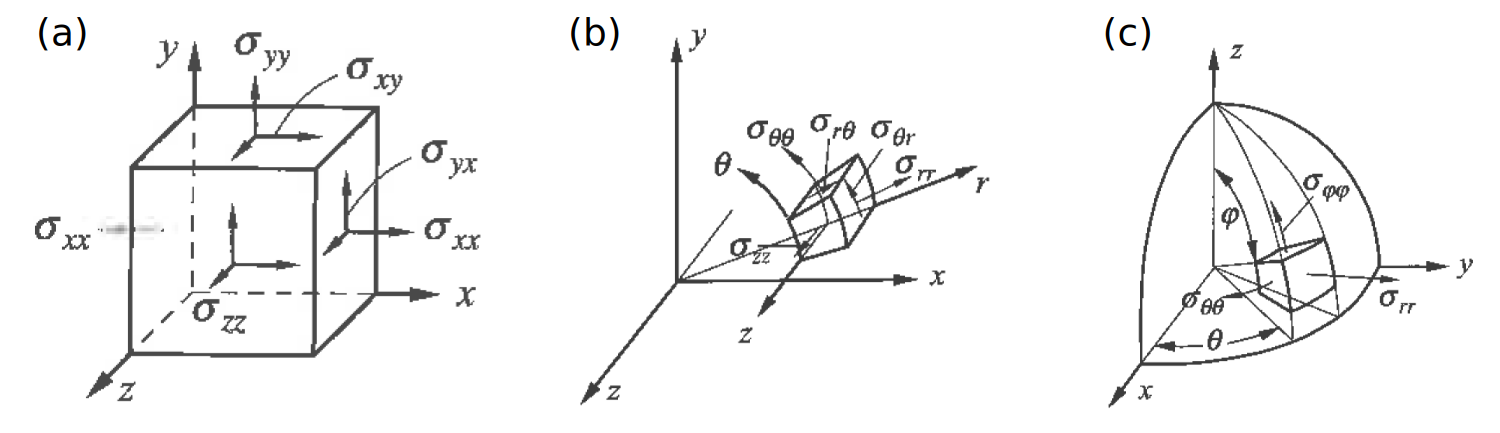
\includegraphics[scale=0.4]{StressTensors}%
	\caption{Stress tensors for (a.) Cartesian, (b.) cylindrical, and (c.) spherical coordinate systems. From Nix and Cai.}%
	\label{fig:StressTensors}%
\end{figure}

\begin{equation}
	\sigma_{ij}
	\begin{bmatrix}
		\sigma_{xx} & \sigma_{xy} & \sigma_{xz}\\
    \sigma_{yx} & \sigma_{yy} & \sigma_{yz}\\
    \sigma_{zx} & \sigma_{zy} & \sigma_{zz}\\
	\end{bmatrix}
	\label{eq:CartesianStressTensor}
\end{equation}

\paragraph{Cylindrical} coordinates are also an orthogonal coordinate system defined in Fig. \ref{fig:StressTensors}(b). The stress tensor in this coordinate system is defined by the cylinderical components $r$, $\theta$, and $z$. Here, $r$ is the distance from the $z$-axis to the point. $\theta$ is the angle between the reference direction (we use the $x$-direction) and the vector that points from the origin to the coordinates projected onto the $xy$ plane. $z$ is the distance from the point's coordinates projected onto $xy$ plane and the point itself. The stress tensor is represented as  

\begin{equation}
	\sigma_{ij}=
	\begin{bmatrix}
		\sigma_{rr} & \sigma_{r \theta} & \sigma_{r z}\\
    \sigma_{\theta r} & \sigma_{\theta\theta} & \sigma_{\theta z}\\
    \sigma_{z r} & \sigma_{z \theta} & \sigma_{zz}\\
	\end{bmatrix}
	\label{eq:CylindricalStressTensor}
\end{equation}

\paragraph{Spherical} coordinates are defined by $r$, $\theta$ and $\phi$. Here $r$ is the radial distance from the origin to the point. $\theta$ is the polar angle, or the angle between the $x$-axis and the point, projected onto the $xy$ plane. $\phi$ is the azimuthal angle, or the angle between the $z$-axis and the vector pointing from the origin to the point. The stress tensor is

\begin{equation}
	\sigma_{ij}=
	\begin{bmatrix}
		\sigma_{rr} & \sigma_{r \theta} & \sigma_{r \phi}\\
    \sigma_{\theta r} & \sigma_{\theta\theta} & \sigma_{\theta \phi}\\
    \sigma_{\phi r} & \sigma_{\phi \theta} & \sigma_{\phi\phi}\\
	\end{bmatrix}
	\label{eq:SphericalStressTensor}
\end{equation}

We will often want to transform tensor values from one coordinate system to another in ${\rm I\!R}^3$. As an example, we will convert the stress state from a cylinderical coordinate system to a Cartesian coordinate system. This transformation from stress state in the original coordinate system ($\sigma_{kl
} = \sigma_{kl}^{r \theta z}$) to the new coordinate system ($\sigma_{ij
}^{'} = \sigma_{ij}^{xyz}$) is performed using the following relationship:

\begin{equation}
	\sigma_{ij}' = Q_{ik}Q_{jk}\sigma_{kl}
	\label{eq:GeneralTransform}
\end{equation}

Where the summation notation (Sec. \ref{sec:SummationNotation}) is implicit. In our example the indices $kl$ indicate the original cylindrical coordinate system ($r$, $\theta$, $z$) and the indices $ij$ indicate the new coordinate system ($x$, $y$, $z$).

Note that Eq. \ref{eq:GeneralTransform} can be written in matrix form as:

\[\sigma = Q \cdot \sigma \cdot Q^{T}\]

The $Q$ matrix is defined the dot products between the unit vectors in the coordinate systems of interest. In simplified 2D transformation from polar to Cartesian, there is no $z$ component in either coordinate system and terms with those indices can be dropped.

%\begin{multline}
	%Q_{ik} \equiv (\hat{e}_{i}^{xyz} \cdot \hat{e}_k^{r \theta z}) =
	%\begin{bmatrix}
		%(\hat{e}_{x} \cdot \hat{e}_{r}) & (\hat{e}_{x} \cdot \hat{e}_{\theta}) & (\hat{e}_{x} \cdot \hat{e}_{z})\\
		%(\hat{e}_{y} \cdot \hat{e}_{r}) & (\hat{e}_{y} \cdot \hat{e}_{\theta}) & (\hat{e}_{y} \cdot \hat{e}_{z})\\
		%(\hat{e}_{z} \cdot \hat{e}_{r}) & (\hat{e}_{z} \cdot \hat{e}_{\theta}) & (\hat{e}_{z} \cdot \hat{e}_{z})\\
	%\end{bmatrix}\\
	%%Q_{jl} \equiv (\hat{e}_{j}^{xyz} \cdot \hat{e}_l^{r \theta z}) \\
%\end{multline}

\begin{equation}
	Q_{ik} \equiv (\hat{e}_{i}^{xy} \cdot \hat{e}_k^{r \theta}) =
	\begin{bmatrix}
		(\hat{e}_{x} \cdot \hat{e}_{r}) & (\hat{e}_{x} \cdot \hat{e}_{\theta})\\
		(\hat{e}_{y} \cdot \hat{e}_{r}) & (\hat{e}_{y} \cdot \hat{e}_{\theta})\\
	\end{bmatrix}\\
	%Q_{jl} \equiv (\hat{e}_{j}^{xyz} \cdot \hat{e}_l^{r \theta z}) \\
\end{equation}

where $\hat{e}_{r}$ and $\hat{e}_{\theta}$ is related geometrically to $\hat{e}_{x}$ and $\hat{e}_{y}$:

\begin{equation}
	\begin{bmatrix}
		\hat{e}_{r} = \hat{e}_{x} \cos(\theta) + \hat{e}_{y} \sin(\theta)\\
		\hat{e}_{\theta} = -\hat{e}_{x} \sin(\theta) + \hat{e}_{y} \cos(\theta)\\
	\end{bmatrix}\\
	%Q_{jl} \equiv (\hat{e}_{j}^{xyz} \cdot \hat{e}_l^{r \theta z}) \\
\end{equation} 

And therefore: 
\begin{align}
	Q_{ik} &\equiv (\hat{e}_{i}^{xy} \cdot \hat{e}_k^{r \theta}) =
	\begin{bmatrix}
		(\hat{e}_{x} \cdot \hat{e}_{r}) & (\hat{e}_{x} \cdot \hat{e}_{\theta})\\
		(\hat{e}_{y} \cdot \hat{e}_{r}) & (\hat{e}_{y} \cdot \hat{e}_{\theta})\\
	\end{bmatrix}
	=
	\begin{bmatrix}
		Q_{xr} & Q_{x\theta}\\
		Q_{yr} & Q_{y\theta}\\
	\end{bmatrix} \\
	&=
		\begin{bmatrix}
		\left(\hat{e}_{x} \cdot \left[\hat{e}_{x} \cos(\theta) + \hat{e}_{y} \sin(\theta)\right]\right) & \left(\hat{e}_{x} \cdot \left[-\hat{e}_{x} \sin(\theta) + \hat{e}_{y} \cos(\theta)\right]\right)\\
		\left(\hat{e}_{y} \cdot \left[\hat{e}_{x} \cos(\theta) + \hat{e}_{y} \sin(\theta)\right]\right) & \left(\hat{e}_{y} \cdot \left[-\hat{e}_{x} \sin(\theta) + \hat{e}_{y} \cos(\theta)\right]\right)	
		\end{bmatrix}\\
		&=
		\begin{bmatrix}
		\cos(\theta) & -\sin(\theta)\\
		\sin(\theta) & \cos(\theta)	
		\end{bmatrix}
\end{align}

So, to convert the stress tensor in polar coordinates ($\sigma_{kl}^{r\theta}$) to Cartesian ($\sigma_{ij}^{xy}$), we take the triple dot-product:

\begin{align}
	\sigma' &= Q \cdot \sigma \cdot Q^{T} =
	\begin{bmatrix}
		\sigma_{xx} & \sigma_{xy}\\
		\sigma_{yx} & \sigma_{yy}
	\end{bmatrix}=
	\begin{bmatrix}
		\cos(\theta) & -\sin(\theta)\\
		\sin(\theta) & con(\theta)	
	\end{bmatrix}\cdot
	\begin{bmatrix}
		\sigma_{rr} & \sigma_{r\theta}\\
		\sigma_{\theta r} & \sigma_{\theta \theta}
	\end{bmatrix}
\cdot
	\begin{bmatrix}
		\cos(\theta) & \sin(\theta)\\
		-\sin(\theta) & con(\theta)	
	\end{bmatrix}
	%&=
	%\begin{bmatrix}
	%\cos(\theta) (\sigma_{rr} \cos(\theta) - \sigma_{\theta r} \sin(\
%\theta)) - \sin(\theta)(\sigma_{r\theta}\cos(\theta) - \sigma_{\theta\theta}\sin(\theta) & \sin(\theta) (\sigma_{rr} \cos(\theta) - \sigma_{\theta r} \sin(\
%\theta)) + \cos(\theta)(\sigma_{r\theta}\cos(\theta) - \sigma_{\theta\theta}\sin(\theta)\\
	%\cos(\theta) (\sigma_{\theta r} \cos(\theta) + \sigma_{rr} \sin(\
%\theta)) - \sin(\theta)(\sigma_{\theta \theta}\cos(\theta) + \sigma_{r\theta}\sin(\theta) & \sin(\theta) (\sigma_{\theta r} \cos(\theta) + \sigma_{rr} \sin(\
%\theta)) + \cos(\theta)(\sigma_{\theta \theta}\cos(\theta) + \sigma_{r\theta}\sin(\theta)
	%\end{bmatrix}
\end{align}

Completing the math yields:
\begin{align}
	\sigma_{xx} &= \cos(\theta) \left[\sigma_{rr} \cos(\theta) - \sigma_{\theta r} \sin(
\theta)\right] - \sin(\theta)\left[\sigma_{r\theta}\cos(\theta) - \sigma_{\theta\theta}\sin(\theta)\right]\\
	\sigma_{xy} &= \sin(\theta) \left[\sigma_{rr} \cos(\theta) - \sigma_{\theta r} \sin(
\theta)\right] + \cos(\theta)\left[\sigma_{r\theta}\cos(\theta) - \sigma_{\theta\theta}\sin(\theta)\right]\\
	\sigma_{yx} &= \cos(\theta) \left[\sigma_{\theta r} \cos(\theta) + \sigma_{rr} \sin(
\theta)\right] - \sin(\theta)\left[\sigma_{\theta \theta}\cos(\theta) + \sigma_{r\theta}\sin(\theta)\right]\\
	\sigma_{yy} &= \sin(\theta) \left[\sigma_{\theta r} \cos(\theta) + \sigma_{rr} \sin(
\theta)\right] + \cos(\theta)\left[\sigma_{\theta \theta}\cos(\theta) + \sigma_{r\theta}\sin(\theta)\right]
\end{align}

In as system with only one or two stress components these coordinate transformations simplify greatly. Remember, though, in ${\rm I\!R}^3$ there will be $N = 3^2$ components due to increased dimentionality.
		
	%Q_{jl} \equiv (\hat{e}_{j}^{xyz} \cdot \hat{e}_l^{r \theta z}) \\

	%\subsubsection{Vector Calculus \hfill(Release TBD)}
	%
	%\textit{\textbf{Encountered in: MAT\texttt{\_}SCI 406, 408}}  \pagebreak
\subsection{Calculus}

We assume that incoming graduate students have completed coursework in calculus including the basic calculation of derivatives, antiderivatives, definite integrals, series/sequences, and multivariate calculus. Below are outlined some more advanced calculus concepts that have specific physical relevance to concepts covered in the MSE core.

Any college-level calculus text is suitable for supplemental study. The sections below on Total Differentials (Sec. \ref{subsec:totdiff}) and Exact/Inexact Differentials (Sec. \ref{subsec:eidiff}) were adapted from the course materials of Richard Fitzpatrick at UT-Austin (available \href{http://farside.ph.utexas.edu/teaching/sm1/Thermal.pdf}{here}).
	
\subsubsection{Total Differentials: \hfill(Release 11/2016)} \label{subsec:totdiff}

\textit{\textbf{Encountered in: MAT\texttt{\_}SCI 401}} 
	
When there exists an explicit function of several variables such as $f = f(x,y,t)$, which has $f$ has a \emph{total} differential of form:
%
\begin{align}
	\Diff{}{f} = \Big(\Partial{}{f}{t}\Big)_{x,y}\Diff{}{t} + \Big(\Partial{}{f}{x}\Big)_{t,y} \Diff{}{x} + \Big(\Partial{}{f}{y}\Big)_{t,x} \Diff{}{y}
\end{align}
%
Here, we do not assume that $f$ is constant with respect any of the arguments $(x\text{,}\, y\text{, or } t)$. This equation defines the differential change in the function $\Diff{}{f}$ and accounts for all interdependencies between $x$, $y$, and $t$. In general, the total differential can be defined as:
%
\begin{align} \label{eq:TotDiff}
	\Diff{}{f} = \sum\limits_{i=1}^n \Big(\Partial{}{f}{x_i}\Big)_{x_{j\neq i}}\Diff{}{x_i}
\end{align}
%
The total differential is important when working with thermodynamic systems which is described by thermodynamic parameters (e.g. $P$, $T$, $V$) which are not necessary independent. For example, the internal energy $U$ for some homogeneous system can be defined in terms of entropy $S$ and volume $V$; $U = U(S,V)$. According to Eq. \ref{eq:TotDiff}, the infinitesimal change in internal entropy is therefore:
%
 \begin{align}
	\Diff{}{U} = \Big(\Partial{}{U}{S}\Big)_{V}\Diff{}{S} + \Big(\Partial{}{U}{V}\Big)_{S} \Diff{}{V}
\end{align}
%
	\subsubsection{Exact and Inexact Differentials \hfill(Release 11/2016)} \label{subsec:eidiff}
	
	\textit{\textbf{Encountered in: MAT\texttt{\_}SCI 401}} 
	
Suppose we are assessing the infinitesimal change of some value: $\Diff{}{f}$, in which $\Diff{}{f}$ is a linear differential of the form:
%
\begin{align}
	\Diff{}{f} = \sum\limits_{i=1}^m M_i(x_1,x_2,...x_m)\Diff{}{x_i}.
\end{align}
%	
In thermodynamics we are often concerned with linear differentials of two independent variables such that 
%
\begin{align} \label{eq:LinearDiff}
	\Diff{}{f} = M(x,y) \Diff{}{x} + N(x,y) \Diff{}{y}.
\end{align}
%
An exact differential is one in which $\int{\Diff{}{z}}$ is path-independent. It can be shown (e.g. \href{http://mathworld.wolfram.com/ExactDifferential.html}{Wolfram Exact Differential}) that this means:
%
\begin{align} \label{eq:ExactDiff}
	\Diff{}{f} = \Big(\Partial{}{f}{x}\Big)_{y} \Diff{}{x} + \Big(\Partial{}{f}{y}\Big)_{x} \Diff{}{y}.
\end{align}
%
Which means that
%
\begin{align} \label{eq:ExactDiff2}
 \Big(\Partial{}{M}{y}\Big)_{x} = \Big(\Partial{}{N}{x}\Big)_{y}. %Wolfram proof.
\end{align}
%
An inexact differential is one in which the equality defined in Eq. \ref{eq:ExactDiff} (and therefore Eq. \ref{eq:ExactDiff2}) is not necessary true. An inexact differential is typically denoted using \textit{bar} notation to define the infinitesimal value:
%
\begin{align}
	\text{\dj} f = \Big(\Partial{}{f}{x}\Big)_{y} \Diff{}{x} + \Big(\Partial{}{f}{y}\Big)_{x} \Diff{}{y}.
\end{align}
%
Two physical examples make this more clear:  %This example is adapted from Safkan on StackExchange. I like it.

\begin{displayquote}
%This example is adapted from Safkan on StackExchange. I like it.
	\textbf{Example 1:} Imagine you are speaking with a classmate who recently traveled from from Chicago to Minneapolis. You know he is now in Minneapolis. Is it possible for you to know how much money he spent gas ($G$)? No, you can't. $G$ is dependent on \emph{how} your friend traveled to Minneapolis: his gas mileage, the cost of gas, and, of course, the route he took. $G$ cannot be known without understanding the details of the path, and is therefore not path independent. The differenitial of $G$ is therefore \emph{inexact}: \text{\dj}$G$.
	
	Now, what do we know about your friend's distance, $D$, to Chicago? This value does not dependent on how he traveled, the only information you need to know is his location, now, in Minneapolis. His distance to Chicago, therefore is a state variable and $\Diff{}{D}$ is an \emph{exact} differential. %Might be better to describe this as a gravitational potential energy, even.
\end{displayquote}

\begin{displayquote}%This example is adapted from Safkan on StackExchange. I like it.
	\textbf{Example 2:} Let's reconsider a situation like that of Example 1 this within the purview of thermodynamics. Consider the internal energy  $U$ of a closed system. To achieve an infinitesimal change in energy $\Diff{}{U}$, we provided a bit of work $\text{\dj}W$ or heat $\text{\dj}Q$:  $\Diff{}{U} = \text{\dj}W + \text{\dj}Q$ \footnote{sometimes, an inexact differential will be denoted as $\delta f$}. The work performed and heat exchanged on the system is path-dependent --- the total work done depends on \emph{how} the work was performed or heat exchanged, and so $\text{\dj}W$ and $\text{\dj}Q$ are inexact.
\end{displayquote}
	
It is sometimes useful to ask yourself about the nature of a variable to ascertain whether the differential is exact or inexact. That is, it makes sense to ask yourself: ``what is the energy of the system?'' or ``what is the pressure of the system''? This often helps in the identification of a state variable. However, it does not make sense to ask yourself ``what is the work of the system'' or ``what is the heat'' of the system --- these values depend on the process. Instead, you have to ask yourself: ``what is the work done on the system along this path?'' or ``what is the heat exchanged during this process?''.

Finally, there are different properties we encounter during the evaluation exact differential (such as the linear differential in Eq. \ref{eq:LinearDiff}), and inexact differentials (written as $\text{\dj}f = M'(x,y) \Diff{}{x} + N'(x,y) \Diff{}{y}$). The integral of an exact differential over a closed path is necessary zero:
%
\begin{align}
	\oint\Diff{}{f} \equiv 0,
\end{align}
%
while the integral of an inexact differential over a closed path is not \emph{necessarily} zero:
%
\begin{align}
	\oint\text{\dj}f\underset{n}{\neq} 0.
\end{align}
%
where $\Big(\underset{n}{\neq}\Big)$ symbolizes ``not necessarily equal to''. Indeed, when evaluating the inexact differential, it is important to consider the path. For example, the work performed a system going from a macrostate $s_i$ to a macrostate $s_2$ is defined by path $L_{1}$, then the total work performed is defined:
%
\begin{align}
	W_{L_{1}} =  \int\limits_{L_{1}} \text{\dj}W
\end{align}
%
If we took a different path, $L_{2}$, the total work performed by be different and
%
\begin{align}
	W_{L_{1}} \underset{n}{\neq}  W_{L_{2}}
\end{align}
%
A good illustration of a line integral over a scalar field is shown in the multimedia Fig. \ref{fig:LineIntegral}. It is clear that, depending on the path, the evaluated integral will have different values.

\begin{figure}%Converted GIF to flv. Some loss in quality. Can embed in YouTube if better.
	\centering
	\includemedia[
		width=0.4\linewidth,
		height=0.3\linewidth,
		activate=pageopen,
		addresource=./Figures/LineIntegralScalarField.flv,
		flashvars={source=./Figures/LineIntegralScalarField.flv}
	]{\includegraphics{./Figures/LineIntegralScalarField.png}}{VPlayer9.swf}
	\caption{An illustration of a line integral along a path in a scalar field, by Lucas V. Barbosa (own work) [Public Domain], via Wikipedia Commons. When using Adobe Pro, allow all multimedia. Click on the figure to run.}%\ref{https://en.wikipedia.org/wiki/Line\_integral\#/media/File:Line\_integral\_of\_scalar\_field.gif}{Wikipedia Commons}
	\label{fig:LineIntegral}%
\end{figure}

	\subsubsection{Vector Calculus \hfill(Release TBD)}
	
	\textit{\textbf{Encountered in: MAT\texttt{\_}SCI 406, 408}}  \pagebreak
\subsection{Differential Equations} \label{sec:DiffEQ}


%\epigraph{Among all of the mathematical disciplines, the theory of differential equations is the most important... It furnishes the explanation of all those those elementary manifestations of nature which involve time.}{\textit{Sophus Lie}}

Differential equations --- equations that relate functions with their derivatives --- are central to the description of natural phenomena in physics, chemistry, biology and engineering. In the sections below, we will outline basic classification of differential equations and describe methods and techniques used in solving equations that are encountered in the MSE graduate core.

The information provide below is distilled and specific to the MSE core, but is by \emph{no means} a equivalent to a thorough 1- or 2-quarter course in ODEs and PDEs. For students who are completely unfamiliar with the material below; i.e., those who have not taken a course in differential equations, we highly recommend enrollment in Applied Math 311-1 and 311-2 \footnote{these may be combined to a 1-quarter class in the future}.

%------------------------------------
	\subsubsection{Classification of Differential Equations \hfill (Release: 11/2016)}
	
	\textit{\textbf{Encountered in: MAT\texttt{\_}SCI 405, 406, 408}} 
	
		Classification of differential equations provide intuition about the physical process that the equation describes, as well as providing context we use as we go about solving the equation. A differential equation can be classified as either ordinary or partial, linear or non-linear, and by its homogeneity and equation order. These are described briefly below, with examples.
		
		\paragraph{Ordinary and Partial Differential Equations ---} The primary classification we use to organize types of differential equations is whether they are \textit{ordinary} or \textit{partial} differential equations. \emph{Ordinary differential equations} (ODEs) involve functions of a single variable. All derivatives present in the ODE are relative to that one variable. Partial differential equations are functions of more than one variable and the partial derivatives of these functions are taken with respect to those variables.
			
An example of an ODE is shown in Eq. \ref{eq:RLC}. This equation has two functions $q(t)$ (charge) and $V(t)$ (voltage), the values of which depend on time $t$. All of the derivatives are with respect the independent variable $t$. $L$, $R$, and $C$ are constants.
%
\begin{align}	
	L \FullDiff{2}{q(t)}{t} + R \FullDiff{}{q(t)}{t} + \frac{1}{C} q(t) = V(t) \label{eq:RLC}
\end{align}
%
This general example describes the flow of charge as a function of time in a \href{https://en.wikipedia.org/wiki/RLC_circuit}{RLC circuit} with an applied voltage that changes with time. Other examples of ODEs you may encounter in the MSE core include ODEs for grain growth as a function of time and the equations of motion.

\emph{Partial differential equations} (PDEs) contain multivariable functions and their partial derivatives i.e., a derivative with respect to one variable with others held constant. As physical phenomenon often vary in both space and time, PDEs --- and methods of solving them --- will be encountered in many of the core MSE courses. These phenomena include wave behavior, diffusion, the Sch\"odinger equation, heat conduction, the Cahn-Hilliard equation, and many others. A typical example of a PDEs you will encounter is Fick's Second Law. In 1D, this is:
%
\begin{align}
	\Partial{}{\varphi(x,t)}{t} = D\Partial{2}{\varphi(x,t)}{x} \label{eq:Ficks2}
\end{align}
%
where $\varphi$ is the concentration as a function of position $x$ and time $t$. This expression equates the change in the concentration over time to the shape (concavity) of the concentration profile. Partial differential equations are, by nature, often more difficult to solve than ODEs, but, as with ODEs, there exist simple, analytic, and systematic methods for solving many of these equations.
			\paragraph{Equation Order ---} The \emph{order} of a differential equation is simply the order of the highest derivative that is present in the equation. In the preceding section, Eq. \ref{eq:RLC} is a second-order equation. Eq. \ref{eq:Ficks2} is also a second-order equation. Students in the MSE core will encounter 4\textsuperscript{th}-order equations such as the Cahn-Hilliard equation, which describes phase separation and is discussed in detail in MAT\texttt{\_}SCI 408. One note concerning notation --- when writing higher-order differential equations it is common to abandon Leibniz's notation (where an $n^{\text{th}}$-order derivative is denoted as $\FullDiff{n}{f}{x}$) in favor of Lagrange's notation in which the following representations are equivalent:
%
\begin{align}
	\text{Leibniz}:& F\big[x,f(x),\FullDiff{}{f(t)}{x},\FullDiff{2}{f(t)}{x}...\FullDiff{n}{f(t)}{x}\big] = 0 \rightarrow\\
	\text{Lagrange}:& F\big[x,f,f\prime,f\prime\prime...f^{(n)}\big] = 0 \label{eq:LagrangeNote}
\end{align}
%
An example would be be the 3\textsuperscript{rd}-order differential equation:
%
\begin{align}
	f\prime\prime\prime + 3f\prime + f\exp{x} = x
\end{align}
%			
			%Add partial differntial notation
%			
			\paragraph{Linearity ---} While considering how to solve a differential equation, it is crucial to consider whether an equation is linear or non-linear. For example, an ODE like that represented in Eq. \ref{eq:LagrangeNote} is linear if the $F$ is a linear function of the variables $f, f', f\prime\prime...f^{(n)}$. This definition also applies to PDEs. The  expression for the general linear ODE of order $n$ is:
%						
\begin{align}
	a_0(x)f^{(n)}+a_1(x)f^{(n-1)} + ... + a_n(x)f = g(t) \label{eq:LinearODE}
\end{align}
%			
Any expression that is not of this form	is considered \textit{nonlinear}. The presence of a product such as $f\cdot f\prime$, a power such as $(f\prime)^2$, or a sinusoidal function of $f$ would make the equation nonlinear.

The methods of solving linear differential equations are well-developed. Nonlinear differential equations, on the other hand, often require more complex analysis. As you will see, methods of \textit{linearization} (small-angle approximations, stability theory) as well as numerical techniques are powerful ways to approach these problems.
			
			\paragraph{Homogeneity ---} Homogeneity of a linear differential equation, such as that shown in Eq. \ref{eq:LinearODE} is satisfied if $g(x) = 0$. This property of a differential equation is often connected to the \textit{driving force} in a system. For example, the motion of a damped harmonic oscillator in 1D (derived from Newton's laws of motion, \href{https://en.wikipedia.org/wiki/Harmonic_oscillator}{here}) is described by a homogeneous linear, 2\textsuperscript{nd}-order ODE:
%			
\begin{align}
	x\prime\prime+2\zeta \omega_0 x\prime \omega_0^2 x = 0
\end{align}
%
where $x = x(t)$ is position as a function of time ($t$) , $\omega_0$ is the undamped angular frequency of the oscillator, and $\zeta$ is the damping ratio. If we add a sinusoidal driving force, however, the equation becomes inhomogeneous:
%
\begin{align}
	x\prime\prime+2\zeta \omega_0 x\prime + \omega_0^2 x = \frac{1}{m} F_0 \sin{(\omega t)} \label{eq:DDSOscillator}
\end{align}
%
One may notice that the form for Eq. \ref{eq:DDSOscillator} is exactly that of the first equation shown in this section (Eq. \ref{eq:RLC}) --- the ODE for a damped, driven harmonic oscillator is exactly the same form as that of the RLC circuit operating under a alternating driving voltage. 
%
	\paragraph{Boundary Conditions ---} Differential equations, when combined with a set of well-posed constraints, or boundary conditions, define a \textit{boundary value problem}. Well-posed boundary value problems have unique solutions from the imposed physical constraints on the system of interest. This analysis allows for the extraction of relevant physical information investigating a physical system --- the elemental composition at some position at time within a diffusion couple, the equilibrium displacement in a mechanically deformed body, or the energy eigenstate of a quantum system. While boundary conditions are not used not classify a differential equation itself, boundary conditions are used to classify the entire boundary value problem --- which is defined by both the differential equation and the boundary value conditions.
	
Boundary value problems are at the heart of physical description in science and engineering. Solving these types of problems allow for the extraction of information (concentration, deformation, stress state, quantum state, etc.) from a system. There are a few types of boundary conditions that you may encounter in the MSE core: %To describe these, we consider a 1D bar of metal which is attached to a heat sink on one side ($x = 0$) and a heater on the other side $x=x_1$. The temperature of the rod is defined as $u(x,t)$. and the temperature behavior of the rod is defined by the heat equation, a homogeneous The %Show in figure.
\begin{enumerate}
	\item A \textit{Dirichlet} (or first-type) boundary condition is one in which specific values are fixed on the boundary of a domain. An example of this is a system in which we have diffusion of carbon (in, for example, a carbourizing atmosphere) into iron (possessing a volume defined as domain $\Omega$) where the carbon concentration $C(\mathbf{r},t)$ at the interface is known for all time $t > 0$. Here, $\mathbf{r}$ is position vector and the domain boundary is denoted as $\partial \Omega$). If this concentration is a known function, $f(\textbf{r},t)$, then the Dirichlet condition is described as:
%	
\[C(\textbf{r},t) = f(\textbf{r},t), \quad	\forall\textbf{r} \in \partial \Omega\] %for t>0? 
%	
	\item A \textit{Neumann} (or second-type) boundary condition is the values of the normal derivative (a directional derivative with respect to the normal of a surface or boundary represented by the vector $\mathbf{n}$) of the solution are known at the domain boundary. Continuing with our example above, this would mean we know the diffusion flux normal to the the boundary at $r$ at all times $t$:
%	
	\[\Partial{}{C(\textbf{r},t)}{\mathbf{n}} = g(\textbf{r},t), \quad	\forall\textbf{r} \in \partial \Omega\] %for t>0? 
%
where $g(\textbf{r},t)$ is a known function, and the bold typesetting denotes a vector.
	\item Two other types of boundary conditions you may encounter are Cauchy and Robin. Cauchy boundary conditions specifies both the solution value and its normal derivative at the boundary --- i.e., it provides both Dirichlet and Neumann conditions. The Robin condition provides a \textit{linear combination} of the solution and its normal derivative and is common in convection-diffusion equations.  
	\item Periodic boundary conditions are applied in periodic media or large, ordered systems. Previously described boundary conditions can therefore combined into periodic sets using infinite sums of sine and cosine functions to create \textit{Fourier series}. This will be discussed in more detail in Sec. \ref{sec:FourierMethods}. 
\end{enumerate}

%	The solution for this equation is the exact		
	\subsubsection{Solving Differential Equations  \hfill (Release: 11/2016)}
	There are many ways to solve differential equations, including analytical and computational techniques. Below, we outline a number of methods that are used in the MSE core to solve relevant differential equations.
		\paragraph{Separation of Variables}, also known as the \textit{Fourier Method}, is a general method used in both ODEs and PDEs to reconstruct a differential equation so that the two variables are separated to opposite sides of the equation and then solved using techniques covered in an ODE class. \label{sec:SepVar} 
		
This method will be used in the solving of many simpler differential equations such as the heat and diffusion equations. These equations must be linear and homogeneous for separation of variables to work. The main goal is to take some sort of differential equation, for example an ordinary differential equation:
%
\begin{align}
	\FullDiff{}{y}{x} &= g(x)h(y)\\
	\intertext{which we can rearrange as:}
	\frac{1}{h(y)}\mathop{dy} &= g(x)dx\\
	\intertext{We now integrate both sides of the equation to find the solution:} 
	\int{\frac{1}{h(y)}\mathop{dy}} &= \int{g(x)\mathop{dx}}
\end{align}	
%
Clearly, we have separated our two variables, $x$ and $y$, to opposite sides of the equation. If the functions are integrable and the resulting integration can be solved for $y$, then a solution can be obtained.

Note here that we have treated the $\mathop{dy}/\mathop{dx}$ derivative as a fraction which we have separated. \ignore{This may bother you (which it should), but it is a useful method which can be validated through \href{https://en.wikipedia.org/wiki/Integration_by_substitution\#Relation_to_the_fundamental_theorem_of_calculus}{integration by substitution}.} 

\begin{displayquote}
	\textbf{Example 1:} Exponential growth behavior can be represented by the equation:
	%
	\begin{align*}
		\FullDiff{}{y(t)}{t} &= k y(t)\\
		\intertext{or}
		\FullDiff{}{y}{t} &= k y\\
		\intertext{This expression simply states that the growth rate of some quantity $y$ at  time, $t$, is proportional to the value of $y$ itself at that time. This is a seperable equation:}
		\frac{1}{y}dy &= k dt\\
		\intertext{We can integrated both sides to get:}
		\int{\frac{1}{y}dy} &= k \int{dt}\\
		\text{ln}(y)+C_1 &= k t + C_2\\
		\intertext{where $C_1$ and $C_2$ are the constants of integration. These can be combined:}
		\text{ln}(y) &= kt+\tilde{C}\\
		y &= e^{(kt+\tilde{C})}\\
		y &= Ce^{kt}
	\end{align*}
	%
	This is clear exponential growth behavior as a function of time. Separation of variables is extremely useful in solving various ODEs and PDEs --- it is employed in the solving of the diffusion equation in \nameref{sec:Sturm-Liouville}.
\end{displayquote}
	
		\paragraph{Sturm-Liouville Boundary Value Problems} \label{sec:Sturm-Liouville}
In this section, we use Sturm-Liouville theory in solving a separable, linear, second-order homogeneous partial differential equation. Sturm-Liouville theory can be used on differential equations (here, in 1D) of the form:
%
\begin{align}
	\FullDiff{}{}{x}\Big[p(x)\FullDiff{}{y}{x}\Big]-q(x)y+\lambda r(x)y = 0 \label{eq:SturmLiouville}
	\intertext{or}
	\big[p(x)y\prime]\prime-q(x)y+\lambda r(x)y = 0 \label{eq:SturmLiouville-2}
\end{align}
%
This type of problem requires knowledge of many use of many concepts and techniques in solving ODEs, including \nameref{sec:SepVar}, Fundamental Solutions of Linear First- and Second-Order Homogeneous Equations, Fourier Series, and Orthogonal Solution Functions. It is important to note that the approach described below (adapted from JJ Hoyt's \textit{Phase Transformations}), which employs separation of variables and Fourier transforms, works only on linear equations. A different approach must be taken for non-linear equations (such as Cahn-Hilliard).

We will use the example of a solid slab of material of length $L$ that has a constant concentration of some elemental species at time zero $ \varphi(x,0) = \varphi_0$ for all $x$ within the slab. On either end of the slab we have homogeneous boundary conditions defining the surface concentrations fixed at $\varphi(0,t) = \varphi(L,t) = 0$ for all $t$. The changing concentration profile, $\varphi(x,t)$ is dictated by Fick's second law, as described earlier in Eq. \ref{eq:Ficks2}:

\begin{equation}	
			\Partial{}{\varphi(x,t)}{t} = D\Partial{2}{\varphi(x,t)}{x} \label{eq:Ficks2-1}
\end{equation}

To use separation of variables, we define the concentration $\varphi(x,t)$, which is dependent on both position and time, to be a product of two functions, $T(t)$ and $X(x)$:

\begin{align}	
	\varphi(x,t) &= T(t)X(x) \label{eq:SepVar-1}
	\intertext{or, in shorthand,}
	\varphi &= TX
\end{align}

It isn't clear why we do this at this point, but stay tuned. Combining Eqs. \ref{eq:Ficks2-1} and \ref{eq:SepVar-1} yields:

\begin{equation}
	XT\prime = DTX\prime\prime
\end{equation}

Where the primed Lagrange notation denotes total derivatives.  $T$ and $X$ are functions only of $t$ and $x$, respectively. Now, we separate the variables completely to acquire:

\begin{equation}
	\frac{1}{DT}T\prime = \frac{1}{X}X\prime\prime
\end{equation}

This representation conveys something critical: each side of the equation must be equal to \emph{the same} constant. This is because the two sides of the equation are equal to each other and the only way a collection of time-dependent quantities can be equivilent to a selection of position-dependent quantities is for them to be constant with respect to both time and position. We select this constant --- for reasons that become clear of the convience of this selection later in the analysis --- as $-\lambda^2$: %Show and example here?
%
\begin{subequations}
	\begin{align}
		\frac{1}{DT}T\prime &= -\lambda^2 \label{eq:SepT}\\
		\frac{1}{X}X\prime\prime &= -\lambda^2 \label{eq:SepX}
	\end{align}  
\end{subequations}	
%
Integration of Eq. \ref{eq:SepT} yields, from \nameref{sec:SepVar}:
%
\begin{align}
	\frac{1}{DT}T\prime &= -\lambda^2 \nonumber\\
	\frac{1}{T}\FullDiff{}{T}{t} &= -\lambda^2 D \nonumber\\
	\int \frac{1}{T}\Diff{}{T} &= -\int \lambda^2 D \Diff{}{t} \nonumber\\
	\ln{T} &= -\lambda^2 D t + T_0 \nonumber\\
	\intertext{where $T_0$ is the combined constant of integration:}
	T = T(t) &= \exp{(-\lambda^2 D t + T_0)} \nonumber\\
	T(t) &= T_0 \exp{(-\lambda^2 D t)} \label{eq:Tt}
\end{align}
%
Eq. \ref{eq:SepX}, on the other hand, is a linear, homogeneous, second-order ODE with constant coefficients that describes simple harmonic behavior. We can solve this by assessing its \href{https://en.wikipedia.org/wiki/Characteristic_equation_(calculus)}{characteristic equation}:
\begin{align}
	r^2+\lambda^2 = 0\\
	\intertext{which has roots:}
	r = \pm \lambda i
\end{align}
When the roots of the characteristic equation are of the form $r = \alpha \pm \beta i$, the \href{http://www.stewartcalculus.com/data/CALCULUS\%20Concepts\%20and\%20Contexts/upfiles/3c3-2ndOrderLinearEqns_Stu.pdf}{solution of the differential equation (Pg. 5)} is:
\begin{equation}
		y = e^{\alpha x}(c_1 \cos{\beta x} + c_2 \sin{\beta x})
\end{equation}

In this instance, $\alpha = 0$ and $\beta = \lambda$, so our solution is:

\begin{equation}
	X = X(x) = \tilde{A} \cos{\lambda x} + \tilde{B} \sin{\lambda x} \label{eq:Xx}
\end{equation}
		
$\tilde{A}$ and $\tilde{B}$ are constants that will be further simplified later. Recalling Eq. \ref{eq:SepVar-1} and utilizing our results from Eqs. \ref{eq:Tt} and \ref{eq:Xx}, we find:
%
\begin{align}
	\varphi(x,y) &= X(x)T(x) = T_0 \big[\tilde{A} \cos{\lambda x} + \tilde{B} \cos{\lambda x}\big]\exp{(-\lambda^2 D t)}\\
	\intertext{where we now define $T_0 \tilde{A} = A$ and $T_0 \tilde{B} = B$ to get:}
	\varphi(x,y) &= X(x)T(x) = \big[A\cos{\lambda x} + B\sin{\lambda x}\big]\exp{(-\lambda^2 D t)} \label{eq:DiffSol}
\end{align}
%
Physially, this solution begins to make sense. At $t=0$ we have a constant concentration, but concentration begins to decay esponentially with time as $D$, $t$, and $\lambda$ are all positive, real constants. The concentration profile is a linear combination of sine and cosine functions, which does not yet yield any physical intuition for this system as we have yet to utilize boundary conditions. 

Recall at this point that we have not specified any value for the constant $\lambda$, as is typical when solving this type of Sturm-Liouville problem. This suggests that there are possible solutions for all values of $\lambda_n$. The Principle of Superposition dictates, then, that if Eq. \ref{eq:DiffSol} is a solution, the complete solution to the problem is a summation of all possible solutions:

\begin{align}
	\Aboxed{\varphi(x,y) = 	\sum_{n=1}^\infty \big[A_n\cos{\lambda_n x} + B_n\sin{\lambda_n x}\big]\exp{(-\lambda_n^2 D t)}} \label{eq:DiffSolFull}
\end{align}

As the value of $\lambda$ influences the values of $A$ and $B$, these values must also be calculated for each $\lambda_n$.

Now, to completely solve our well-posed boundary value problem, we utilize our boundary conditions:
%
\begin{subequations}
	\begin{align}
		\varphi(0,t) &= 0\, \quad t \geq 0 \label{eq:Boundx0}\\
		\varphi(L,t) &= 0\, \quad t \geq 0 \label{eq:BoundxL}\\
		\varphi(x,0) &= \varphi_0\, \quad 0<x<L \label{eq:Time0}
	\end{align}
\end{subequations}
%
At $x = 0$, the sine term in Eq. \ref{eq:DiffSolFull} is zero, and therefore the boundary condition in Eq. \ref{eq:Boundx0} can only be satisfied at all t if $A_n = 0$. At $x = L$, $\sin{\lambda_n x}$ must be zero for all values of $\lambda_n$, therefore $\lambda_n = n\pi/L$. We need only solve now for $B_n$ using the intial condition, Eq. \ref{eq:Time0}.

Using our values of $A_n$ and $\lambda_n$ and assessing Eq. \ref{eq:DiffSolFull} at time $t=0$ yields

\begin{equation}
	\varphi_0 = \sum_{n=1}^\infty B_n \sin{\frac{n \pi x}{L}} \label{eq:Time0-1}
\end{equation}

Here, we must recognized the orthogonal property of the sine function, which states that

\begin{equation}
	\int_0^L \sin{\frac{n \pi x}{L}} \sin{\frac{m \pi x}{L}}
	   \begin{cases}
      = 0, & \text{if}\ n\neq m \\
     \neq 0, & \text{if}\ n = m
    \end{cases}
\end{equation} 

You can test this graphically using a plotting program if you like --- the integrated value of this product is only non-zero when $n=m$ --- or you can follow the proof \href{http://www.math.umd.edu/~psg/401/ortho.pdf}{here}. We can multiply both sides of the Eq. \ref{eq:Time0-1} by $\sin{n \pi x/L}$, then, and integrate both sides from 0 to $L$:
%
\begin{subequations}
	\begin{align}
		\varphi_0 \int_0^L\sin{\frac{m \pi x}{L}} &= \int_0^L \sum_{n=1}^\infty \big[B_n \sin{\frac{n \pi x}{L}} \sin{\frac{m \pi x}{L}}\big] \nonumber
		\intertext{After integration, the only term that survives on the right-hand side is the $m=n$ term, and therefore:}
		\varphi_0 \int_0^L\sin{\frac{n \pi x}{L}} &= B_n\int_0^L \sin{\frac{n \pi x}{L}}^2 \nonumber\\
		\varphi_0 \int_0^L\sin{\frac{n \pi x}{L}} &= \frac{B_n L}{4} \big[2- \frac{\sin{2 n \pi}}{n \pi} \big] \nonumber\\
		\intertext{the $\sin{2 n \pi}$ term is always zero:}
		\varphi_0 \int_0^L\sin{\frac{n \pi x}{L}} &= \frac{B_n L}{2} \nonumber\\
		2 \frac{\varphi_0}{L} \int_0^L\sin{{n \pi x}{L}} &= B_n \nonumber\\
		B_n  &= 2 \frac{\varphi_0}{L} \big[\frac{L}{n \pi}(1-\cos{n \pi})\big] \nonumber\\
		\Aboxed{B_n  &= 2 \frac{\varphi_0}{n \pi} (1-\cos{n \pi})}
	\end{align}
\end{subequations}
%
For even values of $n$, the $B_n$ constant is zero. For odd values of $n$, $B_n = \frac{4 \varphi_0}{n \pi}$. We utilize the values we acquired for $A_n$, $B_n$, and $\lambda$ and plug them into Eq. \ref{eq:DiffSolFull}. A change in summation index to account for the $B_n$ values yields:

\begin{align}
	\Aboxed{\varphi(x,t) = \frac{4 c_0}{\pi} \sum_{k=0}^\infty \frac{1}{2k+1} \sin{\frac{(2k+1)\pi x}{L}}\exp{\Big[-\big(\frac{(2k+1)\pi}{L}\big)^2 Dt\Big]}}
\end{align}

This summation converges quickly. We now have the ability to calculate the function $\varphi(x,t)$ at any position $0 < x < L$ and time $t > 0$!

\newpage
		\paragraph{Method of Integrating Factors} is a technique that is commonly used in the solving of first-order linear ordinary differential equations (but is not restricted to equations of that type). In thermodynamics, it is used to convert a differential equation that is not exact (i.e., path-dependent, See Sec. \ref{subsec:eidiff}) to an exact equation, such as in the derivation of entropy as an exact differential (Release TBD).

\newpage
		\paragraph{Fourier Integral Transforms} \label{sec:FourierMethods}
		This section will introduce an extremely powerful technique in solving differential equations: the Fourier transform. This technique is useful because it allows us to transform a complicated problem --- a boundary value problem --- into a simpler problem which can often be approached with ODE techniques or even algebraically.
		
		There are many excellet sources provided for this section, listed below.
		
		\begin{enumerate}
			\item Jos\'{e} Figueroa-O'Farrill's wonderful \textit{Integral Transforms} from \textit{Mathematical Techniques III} at the University of Edinborough.
			\item W.E Olmstead and V.A. Volpert's \textit{Differential Equations in Applied Mathematics} at Northwestern University.
			\item J.J. Hoyt's chapter on the \textit{Mathematics of Diffusion} in his \textit{Phase Transformations} text.
			\item Paul Shewman's \textit{Diffusion in Solids}.
			\item J.W. Brown and R.V. Churchill's \textit{Fourier Series and Boundary Values Problems}, 6\textsuperscript{th} Edition.
		\end{enumerate}
		
		The primary goal behind the Fourier transform is to solve a differential equation with some unknown function $f$. We apply the transform ($\mathscr{F}$) to convert the function into something that can be solved more easily: $f \xrightarrow{\mathscr{F}} F$. The transformed function is often also represented using a $\hat{f}$. We solve for $F$ and then perform an inverse Fourier transform ($\mathscr{F}^{-1}$) to recover the solution for $f$.
		
		We find that Fourier \textit{series} --- which are used to when working with periodic functions --- can be generalized to Fourier integral transforms (or Fourier transforms) when the period of the function becomes infinitely long. Let's begin with the Fourier series an build on our results from our discussion above where we found that a continuous function $f(x)$ defined on some finite interval $x \in[0,L]$ and vanishing at the boundaries, $f(0) = f(L) = 0$ can be expanded as shown in \ref{eq:DiffSolFull}. 
		
		The following derivation is adapted from Olmstead and Volpert. In general, we can attempt to represent \textit{any} function that is periodic over period $[0,L]$ with a Fourier series of form:

\begin{equation}
f(x) = a_0 + \sum_{n=1}^\infty\left[a_n \cos{\frac{2 \pi n x}{L}} + b_n \sin{\frac{2 \pi n x}{L}}\right]
\label{eq:GenSol}
\end{equation}
		
However, we need to know how to find the coefficients $a_0$, $a_n$, and $b_n$ for this representation of $f(x)$. For this analysis we must utilize the following integral identities:

%Kronecker delta?
%
\begin{equation}
\int_0^L{\sin{\frac{2 \pi n x}{L}}\cos{\frac{2 \pi n x}{L}}}dx= 0 \quad n,m = 1,2,3,...,
\end{equation}

\begin{equation}
\int_0^L{\cos{\frac{2 \pi n x}{L}}\cos{\frac{2 \pi m x}{L}}} dx= 
	\begin{cases}
		0, \text{\,if} \quad n,m = 1,2,3,..., n\neq m\\
		L/2, \text{\,if} \quad n = m = 1,2,3,...,\\
	\end{cases}
\end{equation}

\begin{equation}
\int_0^L{\sin{\frac{2 \pi n x}{L}}\sin{\frac{2 \pi m x}{L}}} dx = 
	\begin{cases}
		0, \text{\,if} \quad  n,m = 1,2,3,..., n\neq m\\
		L/2, \text{\,if} \quad n = m = 1,2,3,...,\\
	\end{cases}
\end{equation}

\begin{equation}
\int_0^L{\cos{\frac{2 \pi n x}{L}}} dx = 
	\begin{cases}
		0, \text{\,if} \quad n,m = 1,2,3,...,\\
		L, \text{\,if} \quad n = 0\\
	\end{cases}
\end{equation}

\begin{equation}
\int_0^L{\sin{\frac{2 \pi n x}{L}}} dx = 
		0, \text{\,if} \quad n,m = 0,1,2,3,...,\\
\end{equation}
		
These identities state  the orthogonal properties of sines and cosines that will be used to derive the coefficients $a_0$, $a_n$, and $b_n$. Recall that two functions are orthogonal on an interval if 

\begin{equation}
\int_a^b f(x)g(x)dx = 0
\end{equation}

We can therefore multiply Eq. \ref{eq:GenSol} by $\cos{\frac{2 \pi x}{L}}$ (note $n = 1$) and integrate over $[0,L]$:

\begin{align}
	\int_0^L f(x)\cos{\frac{2 \pi x}{L}} dx &= a_0 \int_0^L \cos{\frac{2 \pi x}{L}} dx +\\
	&a_1 \int_0^L \cos{\frac{2 \pi x}{L}} \cos{\frac{2 \pi x}{L}} dx +b_1 \int_0^L \sin{\frac{2 \pi x}{L}} cos{\frac{2 \pi x}{L}} dx +\\
	&a_2 \int_0^L \cos{\frac{4 \pi x}{L}} \cos{\frac{2 \pi x}{L}} dx +b_2 \int_0^L \sin{\frac{4 \pi x}{L}} cos{\frac{2 \pi x}{L}} dx + ...\\
\end{align}

Applying the orthogonal properties of the integral products finds that all terms on the right-hand side of this equation are zero apart from the $a_1$ term. The equation therefore reduces to:

\begin{equation}
\int_0^L f(x)\cos{\frac{2 \pi x}{L}} dx = a_1 \int_0^L \cos{\frac{2 \pi x}{L}} cos{\frac{2 \pi x}{L}} dx= a_1\frac{L}{2}
\end{equation}

and 

\[a_1 = \frac{2}{L} \int_0^L f(x)\cos{\frac{2 \pi x}{L}} dx\].

The other Fourier coefficients can be solved for in a similar manner, which yields the general solutions:

\begin{align}
	a_0 &= \frac{1}{L} \int_0^L f(x)\\
		a_n &= \frac{2}{L} \int_0^L f(x)\cos{\frac{2 n \pi x}{L}}dx \quad (n = 1,2,3...)\\
			b_n &= \frac{2}{L} \int_0^L f(x)\sin{\frac{2 n \pi x}{L}}dx\quad (n = 1,2,3...)
\end{align}

To this point we've solved, generally, for the coefficients of a Fourier series over a finite interval. This is useful, but we my want to use the full complex form of the Fourier series in later discussion of the Fourier transform. We know that \href{https://en.wikipedia.org/wiki/Euler's_formula#Relationship_to_trigonometry}{Euler's formula} can be used to express trigonometric functions with the complex exponential function:

\begin{align}
	\sin{\frac{2 \pi n x}{L}} &= \frac{1}{2i}\left(e^{i\frac{n \pi x}{L}}+e^{-i\frac{n \pi x}{L}}\right) \nonumber \\
	\cos{\frac{2 \pi n x}{L}} &= \frac{1}{2}\left(e^{i\frac{n \pi x}{L}}+e^{-i\frac{n \pi x}{L}}\right) \label{eq:Euler}
\end{align}

and we define the wavenumbers to be:

\begin{equation}
	k_n = 2 \pi n/L \quad n=0,1,2,...,
\label{eq:Wavenumber}
\end{equation}

and therefore Eq. \ref{eq:Euler} is written as:

\begin{align}
	\sin{k_n x} &= \frac{1}{2i}\left(e^{i k_n x}+e^{-i k_n x}\right) \nonumber \\
	\cos{k_n x} &= \frac{1}{2}\left(e^{i k_n x}+e^{-i\ k_n x}\right) \label{eq:Euler}
\end{align}

This allows us to write the complete Fourier series (Substitute Eq. \ref{eq:Euler} into \ref{eq:GenSol}): 

\begin{equation}
	f_{L}(x) \sim \sum_{n=-\infty}^{\infty} c_n e^{i k_n x}
\label{eq:ComplexFourierSeries}
\end{equation}

For convenience, we'll define the integral to be $[-\frac{L}{2},\frac{L}{2}]$. The $\sim$ notation indicates that the series representation is an approximation, and the $L$ represents the period over which the series is applied. The orthogonality condition holds for these complex exponential and its complex conjugate over this interval:

\begin{equation}
	\int_{-\frac{L}{2}}^{\frac{L}{2}} e^{i k_n x} e^{-i k_m x} dx =
		\begin{cases}
		0, \text{\,if} \quad n \neq m\\
		L, \text{\,if} \quad n = m\\
	\end{cases}
\end{equation}

Therefore, if we multiply Eq. \ref{eq:ComplexFourierSeries} by $e^{-i k_m x}$ and solve we find the only term that survives is when $n=m$:

\begin{equation}
	\int_{-\frac{L}{2}}^{\frac{L}{2}} f_L(x) e^{-i k_m x} dx = L c_m.
\end{equation}

We can revert the place-keeping subscript $m$ to $n$ and solve for the Fourier coefficients to find:

\begin{equation}
	 c_n = \frac{1}{L}\int_{-\frac{L}{2}}^{\frac{L}{2}} f_L(x) e^{-i k_n x} dx \quad \text{for\,} n = 0, \pm1, \pm2,...
	\label{eq:FourierComps}
\end{equation}

Alright, we've defined an interval $[-L/2, L/2]$, but we want to investigate this interval as $L \rightarrow \infty$ in an attempt to eliminate the periodicity of the Fourier series. If $L \rightarrow \infty$, we know that our function $f_L(x)$ will be non-zero over only a very small range --- say an interval of $[-a/2, a/2]$ where $a << L$. This means that

\begin{equation}
	f_L{x} =
	\begin{cases}
		1 \quad \text{for} |x|<a/2\\
		0 \quad \text{for} a/2 < |x| < L/2
	\end{cases}
\label{eq:Linfty}
\end{equation}

This function is zero except for a small bump at the origin of height 1 and width $a$. Let's assess our function over the non-zero interval:

\begin{equation}
	\int_{-\frac{a}{2}}^{\frac{a}{2}} e^{-i k_n x} dx = \frac{\sin k_n a/2}{k_n L/2} = \frac{\sin n \pi a/L}{n \pi}.
	\label{eq:Thing}
\end{equation}

But how does this allow us to consider a continuous Fourier integral transform? Well, we need to consider the function $f_L(x)$ as $L \rightarrow \infty$. By doing so, we drive all the harmonics of the Fourier function --- apart from the central one --- out beyond infinity. $f(x)$ then has a single bump of width $L$ centered at the origin. That is, the separation between the $n$ harmonics goes to zero, and the representation contains all harmonics. Further, as $L \rightarrow \infty$ we no longer have a periodic function and we can i.e., the fundamental period becomes so large that we no longer have non-periodic function at all. %This needs work

This allows us to transition from a discrete description to a continuum and our Fourier sum can now be described as a Fourier integral. Recall the Fourier series (Eq/ \ref{eq:ComplexFourierSeries}):

\begin{equation}
	f_{L}(x) \sim \sum_{n=-\infty}^{\infty} c_n e^{i k_n x}
\end{equation}

Which we now write as:

\begin{equation}
	f_{L}(x) \sim \sum_{n=-\infty}^{\infty} \frac{\Delta k}{2\pi/L} c_n e^{i k_n x} = \sum_{n=-\infty}^{\infty} \frac{\Delta k}{2\pi} L c_n e^{i k_n x} 
	\label{eq:Thing2}
\end{equation}

where $\Delta k = 2\pi/L$ is the difference between successive values of $k_n$. We now define a function $F(k)$ as

\begin{equation}
	F(k) \equiv \Lim{L \rightarrow \infty} L c_n = \Lim{L \rightarrow \infty} L c_{kL/2 \pi}
	\label{eq:DefFourierTransform}
\end{equation}

Combining this definition with Eq. \ref{eq:Thing} gives:

\begin{equation}
	F(k) = \frac{\sin{(ka/2)}}{k/2}
\end{equation}

and as $L \rightarrow \infty$, Eq. \ref{eq:Thing2} goes as

\begin{align}
	f(x) &= \Lim{L \rightarrow \infty} \sum_{n=-\infty}^{\infty} \frac{\Delta k}{2\pi} L c_n e^{i k_n x} \\
	\Aboxed{f(x) &= \frac{1}{2\pi}\int_{-\infty}^{\infty}F(k) e^{ikx} dk}
\label{eq:FourierInversion}
\end{align}

The function $F(x)$ is the Fourier transform of $f(x)$ and Eq. \ref{eq:FourierInversion} as a continuous superposition of Fourier component, with each component now represented by a \emph{continuous} function $f(x)$. Similarly, from Eq. \ref{eq:DefFourierTransform} and Eq. \ref{eq:FourierComps}:

\begin{align}
	\Aboxed{F(k) &= \int_{\infty}^{\infty} f(x) e^{-i k x} dx}
	\label{eq:FourierTransform}
\end{align}

Eq. \ref{eq:FourierTransform} is non-periodic analog to the expression for deriving the Fourier coefficients $c_n$ in the periodic case. We call this function the \emph{Fourier (Integral) Transform} of the function $f(x)$ and it is often written as 

\begin{equation}
F(k) \equiv \mathscr{F}\big[f(t)\big]
\label{eq:InversionFormula}
\end{equation} 

Similarly, Eq. \ref{eq:InversionFormula} is known as the \emph{Inversion Formula} or \emph{Inverse Fourier (Integral) Transform} and is used to return the Fourier-transformed function from frequency space. It is often represented as:

\begin{equation}
f(x) \equiv \mathscr{F}^{-1}\big[F(k)\big]
\end{equation} 

\begin{displayquote}
	\textbf{Example:} Let's do a simple Fourier transform of a \href{https://en.wikipedia.org/wiki/Square-integrable_function}{square-integrable function} (this condition establishes that the function has a Fourier transform). We'll try a square pulse over the interval [-\pi, \pi]:

	\begin{equation}
		f(x) =
			\begin{cases}
				1, \text{\,if\,} |x| < \pi\\
				0, \text{\,otherwise}\\
			\end{cases}
	\end{equation}

	We take the Fourier integral transform over the non-zero interval:

	\begin{align}
	F(x) &= \frac{1}{2 \pi}\int_{-\infty}^{\infty} f(x) e^{-i k x} dx\\
	&= \frac{1}{2 \pi}\int_{-\pi}^{\pi} e^{-i k x} dx\\
	&= -\frac{1}{2i \pi k} e^{-i k x}\Big|_{-\pi}^{\pi}\\
	&= -\frac{1}{2i \pi k} (e^{-i k \pi}-e^{i k \pi})\\
	&= \frac{\sin{\pi k }}{\pi k}
	\end{align}

	\end{displayquote}

Integral transforms will prove massively useful in solving boundary value problems in the MAT\texttt{\_}SCI core.

\begin{displayquote}
\textbf{Example} One example is diffusion in the thin film problem. Imagine that there is thin region of finite width with high concentration of some species \textbf{B} situated between two ``infinite'' (thick) plate of pure \textbf{A} (after Hoyt, 1-6). Diffusion from the thin film is allowed to proceed over time into the adjacent plates. The thin film is centered at $x = 0$, so the concentration profile will be an even function $[\varphi(x,t) = \varphi(-x,t)]$  How do we solve for the evolution of the concentration profile over time?

This is an example in which we want to interpret this geometry as one with infinite period. When doing so we should consider using a Fourier integral transform.

From the section above, we understand that the concentration profile $c(x,t)$ can be obtained from the inverse transform of the Fourier space function $\Phi(k,t)$. Above, we derived the full Fourier integral transform, but here we know that the function is even, and so we can perform a Fourier Cosine integral transform, which simplifies the mathematics and allows us to perform the transform from $[0,\infty]$. The following derivation is after Hoyt, Ch. 1-8.

\begin{align}
	f(x) = \frac{1}{\pi} \int_{-\infty}^{\infty} F(x) \cos{(kx)} dk\\
	F(x) = \frac{1}{\pi} \int_0^{\infty} f(x) \cos{(kx)} dx
\end{align}

In our case, we have:

\begin{align}
	\varphi(x,t) = \frac{1}{\pi} \int_{-\infty}^{\infty} \Phi(k,t) \cos{(kx)} dk\\
	\Phi(k,t) = \frac{1}{\pi} \int_0^{\infty} \varphi(x,t) \cos{(kx)} dx
	\label{eq:OddSol1}
\end{align}

The utility of utilizing the Fourier intergral transform is that the PDEs in space and time can be converted to ODEs in the time domain alone, which are often much easier to solve. The ability for us to do this hinges on a key property of a Fourier transform that relates the Fourier transform of the $n$\textsuperscript{th} derivative of a function to the Fourier transform of the function itself. 

\begin{equation}
	\mathscr{F}\big[f^{(n)}(x)\big](k) = (ik)^{n}\mathscr{F}\big[f(x)\big](k)
\label{eq:}
\end{equation}

This, as you will see, allows us to convert a PDE in $t$ and $x$ to a ODE in $t$ alone. Let's apply this property to the 1D diffusion equation. First, we know we are performing a Fourier transform in $x$, so the time derivative can be pulled from the integral on the left-hand side of the equation.

\begin{align}
	\mathscr{F}[\Partial{}{\varphi(x,t)}{t}] &= \frac{1}{\pi}\int_{0}^{\infty} \Partial{}{\varphi(x,t)}{t} \cos{(-ikx)} dx\\
	&= \frac{1}{\pi}\Partial{}{}{t}\left[\int_{0}^{\infty}\varphi(x,t)\cos{(-ikx)} dx\right]\\
	&= \frac{1}{\pi}\Partial{}{}{t}\left[\Phi(k,t)\right]
\end{align}

and the right-hand side of the equation is:

\begin{align}
		\mathscr{F}\big[D\Partial{2}{}{x}\varphi(x,t)\big] &= (ik)^2D\mathscr{F}\big[\varphi(x,t)\big]\\
	&= -D\frac{k^2}{\pi}\int_0^{\infty}\varphi(x,t)\cos{(-ikx)} dx\\ 
	&= -D\frac{k^2}{\pi} \Phi(k,t)
\end{align}

and therefore:

\begin{align}
	\frac{1}{\cancel{\pi}}\Partial{}{}{t}\left[\Phi(k,t)\right] &= -D\frac{k^2}{\cancel{\pi}} \Phi(k,t)\\
	\Aboxed{\Partial{}{}{t}\left[\Phi(k,t)\right] &= -Dk^2 \Phi(k,t)}
\end{align}

This differential equation can be solved by inspection\footnote{If you don't see this, that's fine, review \textit{Separation of Variables} --- this equation is separable} to be:

\begin{equation}
	\Phi(k,t) = A^{0}(k) e^{-k^2Dt}
	\label{eq:Sol1}
\end{equation}

Where $A^0(k)$ is a constant that that defines the Fourier space function $\Phi$ at $t=0$. To fully solve this problem and derive $\varphi(x,t)$ we must next solve this value $A^0(k)$ and apply the inverse Fourier transform.

Let us consider our initial condition. Our concentration profile can be modeled as a $delta$-function concentration profile, $\varphi(x,0) = \alpha \delta(x)$) fixed between two infinite plates, where the integrated concentration is $\alpha$:

\begin{equation}
	\int_{\infty}^{\infty} \varphi(x,0)dx = \int_{\infty}^{\infty} \alpha \delta(x) dx = \alpha
\end{equation}

The constant $A^0(k)$ is, at $t = 0$, defined by Eq. \ref{eq:Sol1} and Eq. \ref{eq:OddSol1}  to be:

\begin{align}
	\Phi(k,t) &= A^{0}(k)e^{0}\\ 
	&= \frac{1}{2\pi}\int_{0}^{\infty}\varphi(x,t) \cos{(kx)} dx
\end{align}

Inserting the delta function for \varphi(x,t) yields:

\begin{equation}
	A^{0}(k) = \frac{\alpha}{\pi}\int_{0}^{\infty} \delta(x) \cos{(kx)} dx
\end{equation}

We'll take advantage of the evenness of this function and instead integrate over $[\infty, \infty]$. This allows us to avoid the messiness at $x=0$ as well circumvent using the Heaviside step function.

\begin{align}
	A^{0}(k) &= \frac{\alpha}{2\pi}\int_{-\infty}^{\infty} \delta(x) \cos{(kx)} dx\\
	A^{0}(k) &= \frac{\alpha}{2\pi} \cos{(0)} dx\\ %Deltafunction fundamental property
	\Aboxed{A^{0}(k) &= \frac{\alpha}{2\pi}}
\end{align}

Finally, now that we have $A^{0}$, we must perform the inverse transformation to find the expression for $\varphi(x,t)$.

\begin{align}
	\varphi(x,t) &= \frac{\alpha}{2\pi}\int_{-\infty}^{\infty} e^{-k^2Dt} \cos{(kx)} dk\\
	\intertext{This can be completed through integration by parts, trigonometric identities, and completing the square... for explicit step-by-step analysis use Wolfram$|$Alpha or \href{http://www.integral-calculator.com/}{Scherfgen's Integral Calculator}. Let's state the result:}
	\varphi(x,t) &= \frac{\alpha}{2\sqrt{\pi D t}} e^{-x^2/4Dt}
\end{align}

This is a Gaussian distribution centered at $x = 0$ and which increases in width with time. This is good --- it certainly makes sense intuitively.

	%\intertext{say:} 
	%u = e^{-k^2Dt} \quad du &= 2kDt e^{-k^2Dt}dk\\ 
	%v = \frac{1}{x}\sin(kx) \quad dv &= \cos{(kx)}dk\\
	%\int e^{-k^2Dt} \cos{(k x)}dk &= e^{-k^2Dt} \frac{1}{x}\sin{(kx)} - 2kDt \int e^{-k^2Dt} \sin{(x)}dk\\
%\end{align}

\end{displayquote}	
	
\paragraph{Bessel Functions}
\paragraph{Legendre Polynomials}
\paragraph{Euler's Method}
\subsubsection{Solving Second-order Linear ODEs \hfill (Release TBD)}
	\begin{enumerate}
		\item Principle of Superposition
		\item Series Solutions
	\end{enumerate}
\subsubsection{Laplace Transforms \hfill (Release TBD)}
\subsubsection{Stability Theory \hfill (Release TBD)} \pagebreak
%\input{./Mathematics/Complex Functions} \pagebreak

